\graphicspath{{chapters/notes/03/images}}
\chapter{Genetic Fingerprinting}

\section{Introduction}
Genetic fingerprinting is a technique used to investigate some characteristics of a genome, typically a pattern of variable elements, like SNPs or minisatellites, in order to uniquely characterize a genome.
It can be used to compare a genome with a reference sample or to compare different genomes between each other in order to determine their diversity or analogy.

	\subsection{Fields of interest}
	DNA fingerprinting is used in different fields, like:

	\begin{multicols}{2}
	\begin{itemize}
			\item In forensics for identification purposes.
			\item In lineage related tests, for cells or humans like paternity or hereditary tests.
			\item For the certification of the origin of cells used in the laboratory, to make sure that the cells are the right ones and that there are no major genetic drifts.
				It is necessary when using certain cell lines in an experiment for publishing purposes.
			\item To identify and remove samples that would skew the data.
				For example members of the same family when performing a GWAS study on a certain geographic area.
		\end{itemize}
	\end{multicols}

	\subsection{Variants used for genetic testing}
	Different variants can be used for genetic fingerprinting, such as Single Nucleotide Polymorphisms (SNPs) or inherited Copy Number Variations (CNVs).
	In the past, before sequencing and SNPs array, short tandem repeats were commonly used for genetic fingerprint.

		\subsubsection{CNVs}
		CNVs are a phenomenon in which sections of the genome are repeated or deleted, changing the number of times those regions appear in the genome.
		The most amenable type of inherited CNVs for genetic fingerprinting are the loss-CNVs.
		For a loss CNV in the population the copy number can vary between $2$ and $0$.
		In particular if both parents are heterozygous for a particular CNV their offspring could have an homozygous deletion.
		If instead both parents have $2$ copies at a site that is polymorphic in the population, all of their offspring will have a copy number of $2$.
		Gain-CNVs are difficult to analyse for this tests because when combining multiple copies the origin of a single copy number cannot be traced to a parent and so they cannot be used for genetic fingerprinting.

		\subsubsection{SNPs}
		SNPs are substitutions of a single nucleotide at a specific position in the genome.
		They are the most amenable type of variation as they are simple, abundant in the genome and easy to detect in sequencing data even with low coverage.
		For these reasons the focus of this work will be on SNP-based genetic tests.


\section{SNPs features}

	\subsection{Hardy-Weinberg equilibrium}
	One property of SNPs which has to be taken into account when using them for genetic testing is the Hardy-Weinberg equilibrium.
	In population genetics, the Hardy-Weinberg equilibrium states that allele and genotype frequencies in a population will remain constant from generation to generation under neutral selection, so in the absence of other evolutionary influences, like:

	\begin{multicols}{4}
		\begin{itemize}
			\item Genetic drift.
			\item Mate choice.
			\item Sexual selection.
			\item Mutation.
		\end{itemize}
	\end{multicols}

	In the simplest case of a single locus with two alleles denoted $A$ and $a$ with frequencies $f(A) = p$ and $f(a) = q$ in a population the expected genotype frequencies under random mating are:

	\begin{multicols}{3}
		\begin{itemize}
			\item $f(AA) = p^{2}$ for $AA$ homozygotes.
			\item $f(aa) = q^{2}$ for $aa$ homozygotes.
			\item $f(Aa) = 2pq$ for $Aa$ heterozygotes.
		\end{itemize}
	\end{multicols}

	In the absence of selection, allele frequencies $p$ and $q$ are constant between generations, reaching an equilibrium.
	The general equation that the allele frequencies need to fit in to be considered in equilibrium is:

	$$( P + Q )^2 = 1 \qquad\land\qquad P^2 + 2PQ + Q^2 = 1$$

	SNPs that respect this equilibrium are the most studied and thus the most informative.

	\subsection{Minor allele frequency}
	Minor allele frequency is the frequency at which the second most common allele occurs in a given population.
	When performing genetic fingerprinting, the aim is to maximize the probability to have different genotypes in unrelated individuals.
	For this reason, the more advantageous SNPs will be the ones in which the allelic frequency of the variants is the highest possible.
	Highest variability in the population allows to distinguish better more individuals.

		\subsubsection{Optimal MAF values for genetic fingerprinting}
		Number-wise, a frequency of $\frac{1}{3}$ for each SNP would maximize the variability in a population, but those SNPs wouldn't be in Hardy-Weinberg equilibrium generating possible missed calls.
		Therefore, the optimal SNPs to detect individuals’ differences and similarities are those with genotype frequencies:

		\begin{multicols}{3}
			\begin{itemize}
				\item $P_{AA} = 0.25$.
				\item $P_{BB} = 0.25$.
				\item $P_{AB} = 0.5$.
			\end{itemize}
		\end{multicols}

		So the best SNPs will be those with $MAF = 0.5$.

	\subsection{Haplotype blocks}
	Another important feature to consider for SNPs selection are Haplotype blocks.
	They are blocks along the genome that tend to be inherited together as segments.
	In these regions there is little evidence for historical recombination and only a few common haplotypes are observed.
	Because of this to perform genetic fingerprinting it is enough to consider only a SNPs per haplotype block because the other won't bring additional information.

		\subsubsection{Linkage disequilibrium}
		SNPs in the same HB are said to be in Linkage Disequilibrium (LD).
		Linkage disequilibrium is a measure of the non-random associations between alleles or polymorphisms at different loci.
		A higher LD indicates SNPs with a stronger tendency to co-segregate.
		Haplotype Blocks are therefore commonly represented with linkage disequilibrium plots like the one in figure \ref{fig:linkage}.
		In these plots, SNPs are represented in a way that does not respect the genomic distance, but the order along the genome or the position of each SNP relative the others.

		\begin{figure}[H]
			\centering
			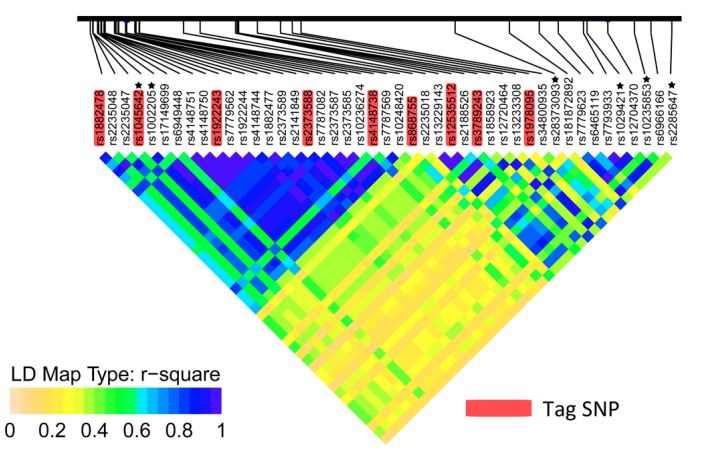
\includegraphics[width=0.7\textwidth]{linkage.png}
			\caption{\label{fig:linkage}LD plot of SNPs with top-ranked bayes factors in CHB (Han Chinese in Beijing) of 1000 Genome Phase I. The colors indicate the strength of pairwise LD according to $r2$ metrics. The SNPs marked with asterisks represent independent strong associations. Tag SNPs are here shadowed in pink.}
		\end{figure}

		The colors indicate the strength of pairwise linkage disequilibrium (LD) according to the $r2$ metrics, the proportion of the variation in the dependent variable that is predictable from the independent ones.
		In fact, not all of the SNPs are informative to distinguish between individuals.

		\subsubsection{Tag SNPs}
		In figure \ref{fig:linkage} tag SNPs are shadowed in pink.
		A tag SNP is representative of a region with high linkage disequilibrium and represents a group of SNPs or haplotype.
		This tag SNPs are the ones that will be included in a genetic fingerprinting test.

	\subsection{Other SNP features}
	Other SNP features to take into consideration when performing a genetic fingerprinting test are:

	\begin{multicols}{2}
		\begin{itemize}
			\item Exclude chromosomal locations which undergo frequent somatic aberrations.
				For example areas commonly deleted in tumour will produce LOH but probably also no calls, since there is no DNA to be sequenced.
			\item Choose SNPs equally spread all around the genome so to represent it all.
			\item Select only autosomal SNPs.
			\item Select SNPs in exons, so to have signal even from a non-DNA assay.
			\item Exclude or include disease or drug response associated loci.
			\item Include or exclude loci with significantly different MAF in different ethnicity.
				Including them allow to perform a lineage test in the same assay.
		\end{itemize}
	\end{multicols}

	\subsection{Number of SNPs to select when performing a genetic test}
	The number of SNPs needed to run a genetic fingerprinting test must be assessed.
	This number should be allow the measure of the test to differentiate unrelated individuals.
	When choosing this number experimental and biological mismatches must be taken into account, weighted based on their likelihood.
	When choosing the number of SNP all the possible mismatches must be taken into account, increasing it to allow to identify individuals.

		\subsubsection{Experimental mismatches - Genotype call error rate}
		During sequencing errors can occur, resulting in no data available for some loci, that if they include SNPs of interest will cause a loss of a call for that SNP.
		These experimental mismatches are related to the error rate of the technology used and because of this they are platform dependent.

			\paragraph{An example on the effect of experimental mismatches}

			\begin{figure}[H]
				\centering
				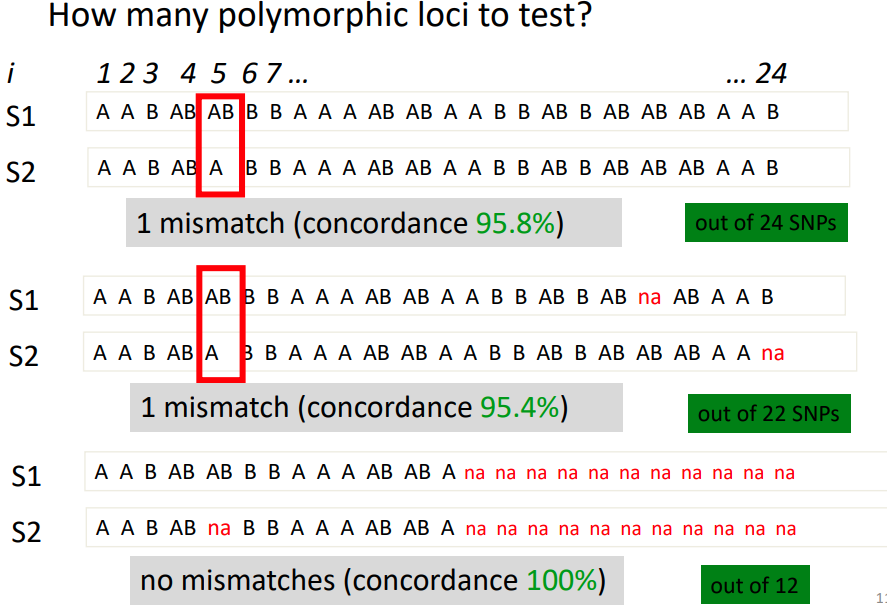
\includegraphics[width=0.6\textwidth]{SNP.PNG}
				\caption{Effect of the error rate on concordance}
				\label{fig:SNP}
			\end{figure}

			In each example in figure \ref{fig:SNP} two sample for which $24$ SNPs are called are analysed.
			To determine the difference of the two samples genotype for each position is considered and mismatches counted.
			In the figure:

			\begin{multicols}{3}
				\begin{itemize}
					\item 'A' stands for homozygous for the reference.
					\item 'B' stands for homozygous for the alternative.
					\item 'AB' stands for heterozygous.
				\end{itemize}
			\end{multicols}

			Analysing now SNPs calls:

			\begin{multicols}{2}
				\begin{itemize}
					\item In the first test over the $24$ loci, there is only one mismatch.
						The level of concordance is $95.8\%$.
						So the individual are highly related or the DNA come from the same sample.
					\item In the second test there is only one mismatch but there are position without a call.
						Therefore the concordance is measured out of $22$ SNPs and is equal $95.4\%$.
					\item In the third test there are a lot of missing calls, so only $12$ SNPs are available and concordance is $100\%$.
				\end{itemize}
			\end{multicols}

			This different level of concordance is due to missing calls in the second and third test.
			The first is the most accurate as it considers the greater number of SNPs between the three, providing the most reliable information.

		\subsubsection{Biological mismatches}
		In the context of disease samples and tumours, many somatic events can happen, like deletions, gains of copies or homozygous deletions.
		This events can change the genetic make-up of a person and have to be taken into account when performing a genetic test.

			\paragraph{Loss of Heterozygosity (LOH)}
			LOH is an event that results in the loss of one parental copy of a region which results in the genome having just one copy of that region.
			If that region contained a heterozygous locus, there will be loss of heterozygosity.
			Its probability of arising is:

			$$P(AB, A) = P(AB)\cdot P(A|AB)$$

			\paragraph{Gain Of Heterozygosity (GOH)}
			GOH is due to a mutation in a site.
			It is polymorphic through inheritance.
			These types of events are pretty rare and their probability of arising is:

			$$P(A,AB) = P(A) \cdot P(AB | A)$$

			\paragraph{Double Mutation (DM)}
			Double mutations are event when a mutation occurs on an already mutated event.
			They are very rare and their probability of arising is:

			$$P(A,B) = P(A) \cdot P(B | A)$$

			\paragraph{Modelling biological mismatches}
			Biological mismatches can be modelled in an assay in a data driven way, assessing the error rate for genotyping for some specific SNPs or running specific tests.
			The resolution for the errors of these mismatches can be patient-wide or tissue-specific.


	\subsection{Project regarding SNPs}
	Some useful projects developed over the years are:

	\begin{multicols}{2}
		\begin{itemize}
			\item dbSNPs.
			\item HapMap3.
		\end{itemize}
	\end{multicols}

		\subsubsection{dbSNPs}
		dbSNPs is a database of small scale nucleotide variants.
		It includes both common and rare single base nucleotide variation (SNV), short ($\leq$ 50bp) deletion/insertion polymorphisms, and other classes of small genetic variations.
		It can be found on \url{https://www.ncbi.nlm.nih.gov/snp/}.

		\subsubsection{HapMap3}
		HapMap3 is the third phase of the HapMap project whose aim is to develop a haplotype map of the human genome to describe the common patterns of human genetic variation in order to allows researchers to find genes and genetic variations that affect health, disease and individual responses to medications and environmental factors.
		The HapMap is a catalog of common genetic variants that occur in human beings.
		It describes what these variants are, where they occur in our DNA, and how they are distributed among people within populations and among populations in different parts of the world.
		It can be found on \url{https://www.sanger.ac.uk/resources/downloads/human/hapmap3.html}

\section{Genetic distance}
Having defined the number of SNPs to use, with maximum MAF and other amenable characteristics, the genetic test should provide a measure of the genetic distance between individuals associated with a probability of the measure to be correct.

	\subsection{Measuring distance}
	As a simple measure, the number of loci where two samples show different genotype can be counted and normalized on the total number of queried loci, defining a certain level of discordance.
	The output value will be the genetic distance between the two samples given the selected loci, which will be proportional to the number of discordant calls.
	In figure \ref{fig:Distance} a typical graph used to measure the genetic distance using SNP-based genetic testing is depicted.
	$4$ samples with a set of $5$ SNPs for each one are analysed.
	The distance is measured among all possible pairs, whose indexes are reported on the x-axis.

	\begin{figure}[H]
		\centering
		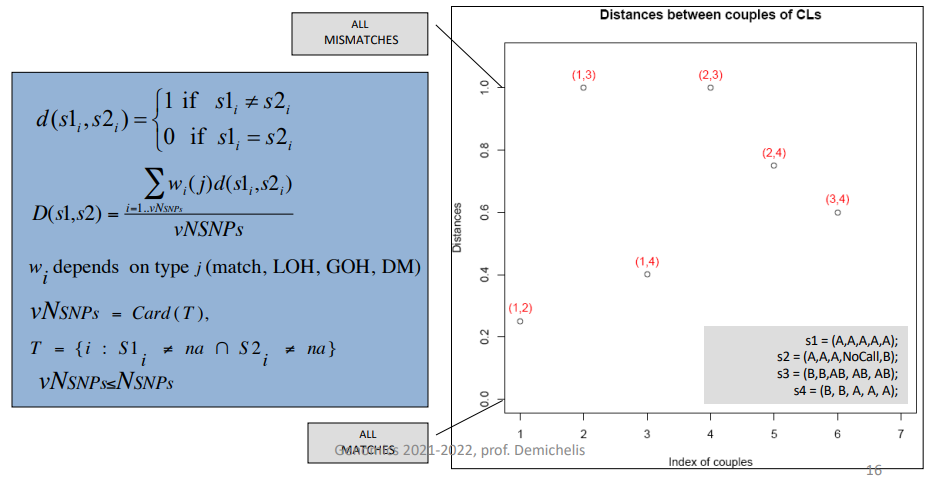
\includegraphics[width=0.7\textwidth]{loci.PNG}
		\caption{Genetic Distance graph with 4 samples. On the y axis the genotype distance is represented, varying from $0$, total concordance to $1$ total discordance. On the x-axis all possible pairs in the dataset are included.}
		\label{fig:Distance}
	\end{figure}

	In particular in figure \ref{fig:Distance}:

	\begin{multicols}{2}
		\begin{itemize}
			\item $s1$ and $s2$ have $3$ equal calls, one locus without call and a mismatch.
				The genetic distance is $0.25$.
			\item Samples $s1$ and $s3$ have $5$ mismatches out of $5$ SNPs, so the genetic distance is $1$.
		\end{itemize}
	\end{multicols}

	The equation in \ref{fig:Distance} is the one used to compute genetic distance.
	The weight $w_i$ can be used to associate different importance to different mismatches.
	The distance is normalized by the total number of SNPs for which there are available calls $vNSNPs$, such that $vNSPNs\le NSNPs$, the total number of SNPs considered in the test.

		\subsubsection{Expected distance}

		\begin{figure}[H]
			\centering
			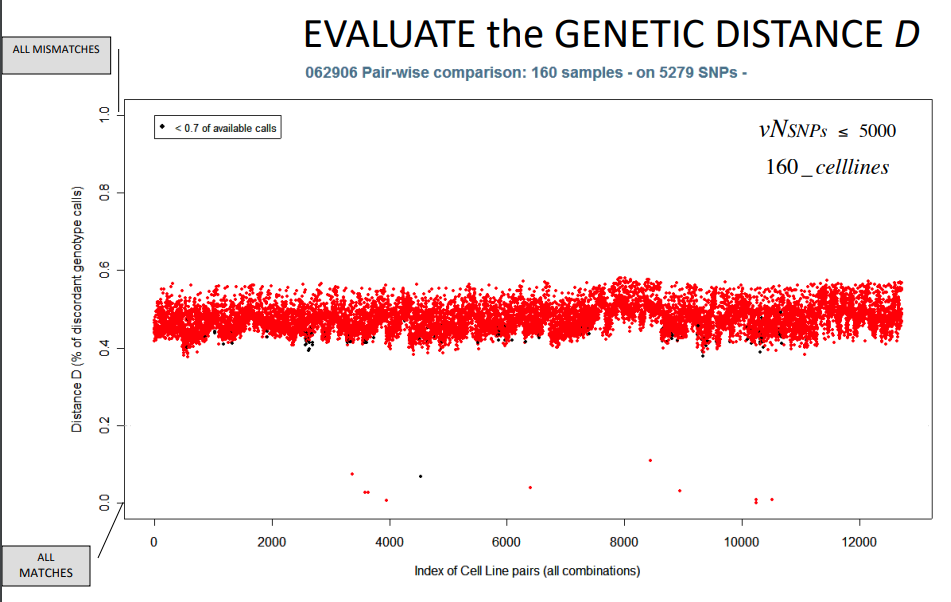
\includegraphics[width=0.7\textwidth]{loci2.PNG}
			\caption{Genetic Distance graph with 160 samples}
			\label{fig:Distance2}
		\end{figure}

		Figure \ref{fig:Distance2} shows the distance, measured by genetic fingerprinting, of a collection of 160 samples of cell lines.
		There are $\frac{160\cdot159}{2}$ possible pairs.
		Applying the distance measure to a larger collection of samples an average distance among all possible pairs is expected.
		This, for different samples will be close to $1$, never reaching it due to genetic variance and errors.
		In this case the average distance is around $0.5$, since by chances some samples share some genotypes.
		Some pairs have a low distance: this is due to a mislabelling to the cell lines used: some believed to be two different cell lines were in fact the same one.

		\subsubsection{Identifying a sample origin from RAP samples}

		\begin{figure}[H]
			\centering
			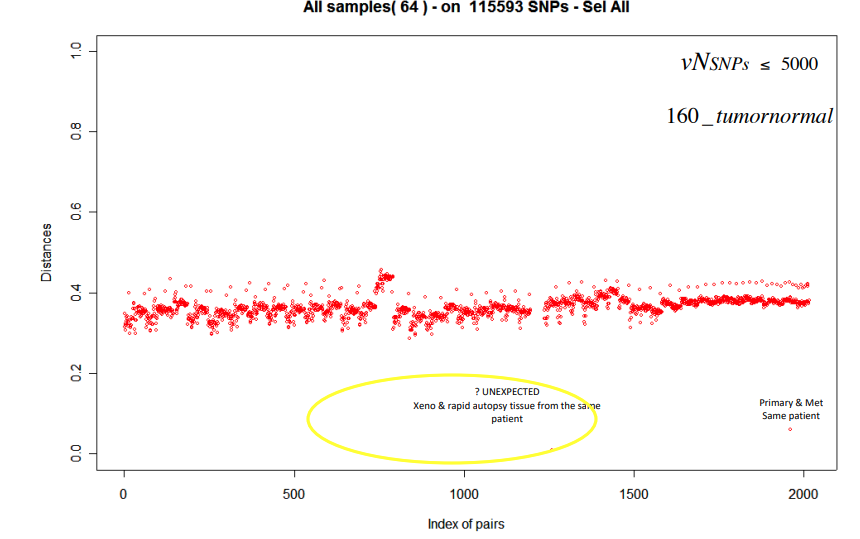
\includegraphics[width=0.7\textwidth]{loci3.PNG}
			\caption{Genetic Distance graph with tumour samples}
			\label{fig:Distance3}
		\end{figure}

		Figure \ref{fig:Distance3} depicts a genetic fingerprinting experiment performed on a collection of $160$ tumour samples, with a SNP array composed of more thant $100000$ SNPs.
		Two samples with very low distance can be observed.
		One of the is from a Rapid Autopsy program and the other from a xenograft model.
		Rapid autopsy programs or	RAP are programs for which patients at the end of their life agree to donate their tumour tissues for research purposes.
		The material must be taken within two hours after death.
		Those sample are usually highly characterized but the patient's identity is lost.
		So the metastasis model used for the xenograft was the one obtained from the RAP.

	\subsection{Distance changes with different numbers of SNPs}

	\begin{figure}[H]
		\centering
		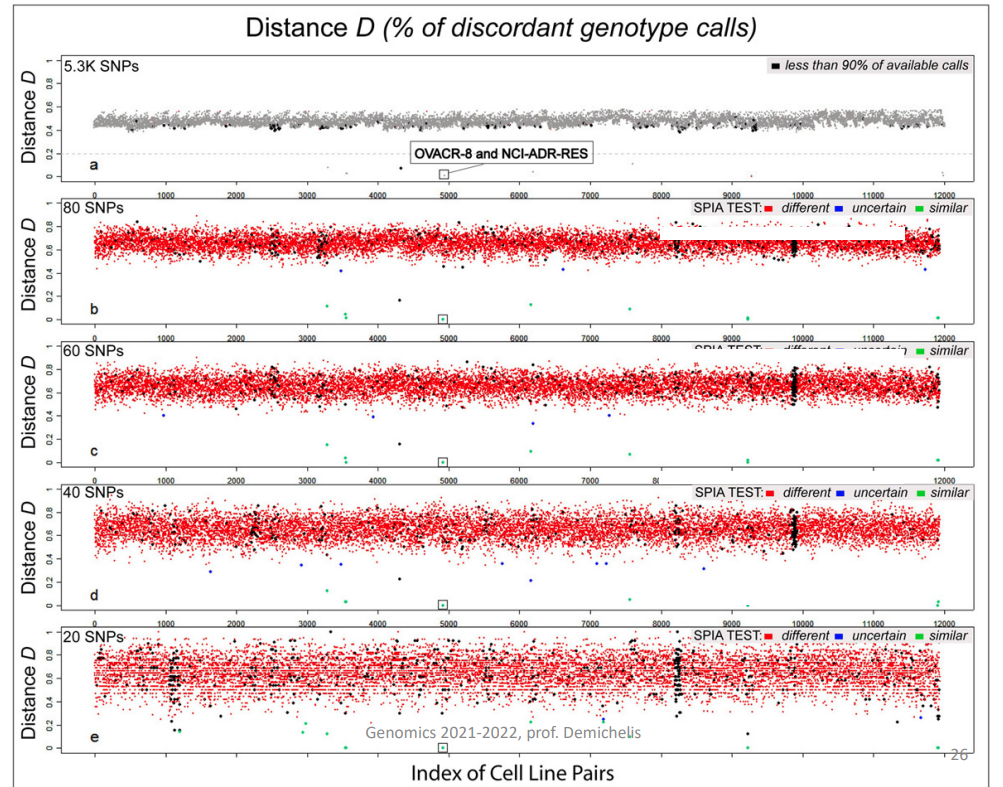
\includegraphics[width=0.7\textwidth]{selected.PNG}
		\caption{Genetic Distance graph at decreasing number of selected SNPs}
		\label{fig:sel_snp}
	\end{figure}

	Figure \ref{fig:sel_snp} depicts an experiment in which the genetic distance among many samples, with an array of $5.3K$ SNPs, was measured using a decreasing number of SNPs from the initial total number of SNPs to decreasing numbers of highly selected SNPs.
	It is noticeable that, in the second plot where $80$ SNPs matching the required characteristics were selected, the average distance and the standard deviation across all pairs is higher than in the previous example, in which all available SNPs were used.
	Decreasing the number of SNPs to 60, then to 40 and 20 leads to have the same average distance between pairs, which settles around 0.66, but higher standard deviation.
	So enough SNPs in order to prevent unexpected issues and to trust the measure are needed.
	Maximizing the likelihood that SNPs have a different genotype, the average distance of unrelated individuals will increase.

\section{Building a SNP-based genetic test}

	\subsection{Pipeline}
	Building an identity test base on SNPs is a multi-step process, consisting in:

	\begin{multicols}{2}
		\begin{enumerate}
			\item Definition of a genetic distance to compare samples.
			\item Definition of SNPs requirements, based on the intention of the assay.
			\item Selection of SNPs:
			\begin{itemize}
				\item This can be done in a data-driven manner, through an iterative procedure of training and test on known sample set;
				\item MAF and Hardy-Weinberg equilibrium from HapMap data.
			\end{itemize}
			\item Implementation of a probabilistic test of classification.
			\item In silico validation on independent datasets.
			\item Validation on cell lines genotyped on independent platform.
		\end{enumerate}
	\end{multicols}

	\subsection{Implementation of a probabilistic test to identify samples}
	When classifying samples there is a need to assess the threshold on the genotype distance to assign samples to a class, the confidence of the classification and the minimum number of loci needed for a robust test.
	A probabilistic test could be used to define the threshold and the confidence.
	The gold standard to do so is to compare observation with expectations.
	Assuming that SNP calls at different loci are independent, this process can be modelled as a binomial distribution: each SNP call is a trial, with $n$ the number of SNPs in the assay, $k$ the number of matches, $p$ the probability of a match and $1-p$ the probability of a mismatch.
	The probability of having $k$ matches out of $n$ SNPs follows a binomial distribution.
	Moreover with $n$, $np$ and $np(1-p)$ large enough, the Gaussian approximation of the binomial distribution can be used.
	Doing so the probability of having $k$ matches out of $n$ SNPs can be modelled as a Gaussian distribution with:

	$$\mu = np\qquad\land\qquad \sigma = np(1-p)$$

	The area of confidence o the assay can be defined as $1m\pm m\cdot \sigma$, where $m$ is the number of standard deviations used to define the threshold.

		\subsubsection{Classification}

		\begin{figure}[H]
			\centering
			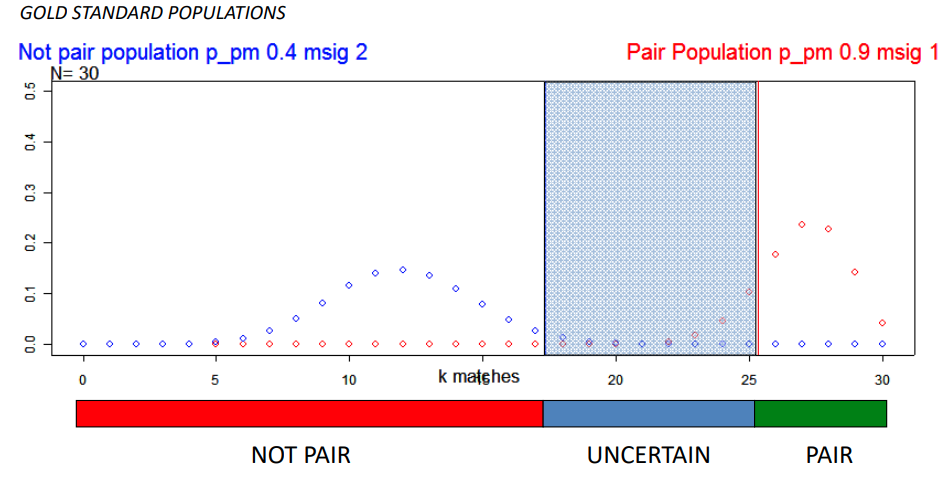
\includegraphics[width=0.7\textwidth]{double_test.PNG}
			\caption{}
			\label{fig:prob_test}
		\end{figure}

		Having modelled the match distribution, the probability mass function for unrelated individual (blue dotted line in figure \ref{fig:prob_test}) can be plotted
		The same can be done with the probability mass function for related individual (red dotted line in figure \ref{fig:prob_test}).
		These functions can be used to set thresholds to define $3$ regions dependent on the number of matche:

		\begin{multicols}{3}
			\begin{itemize}
				\item Not pair: samples in this region are different.
				\item Pair: samples in this regions are similar.
				\item Uncertain: no certain result.
			\end{itemize}
		\end{multicols}

		The grey area changes with $m$ and defines the level of confidence.
		Decreasing the number of SNPs the grey zone will decrease, making the results difficult to interpret.

	\subsection{Some examples of genetic tests}

		\subsubsection{Investigating cell line passages}
		A massive use of these genetic tests is done to assess genetic changes during in-vitro cultivation  and in studies for tumor evolution, lineage plasticity and heterogeneity across metastasis across individuals or in single tumor.
		Cell lines go through multiple passages in which they are used and stored.
		Genetic fingerprinting can be used to assess if among different passages the cells have remained the same, if they were mislabeled or if major genetic drifts happened.

		\begin{figure}[H]
			\centering
			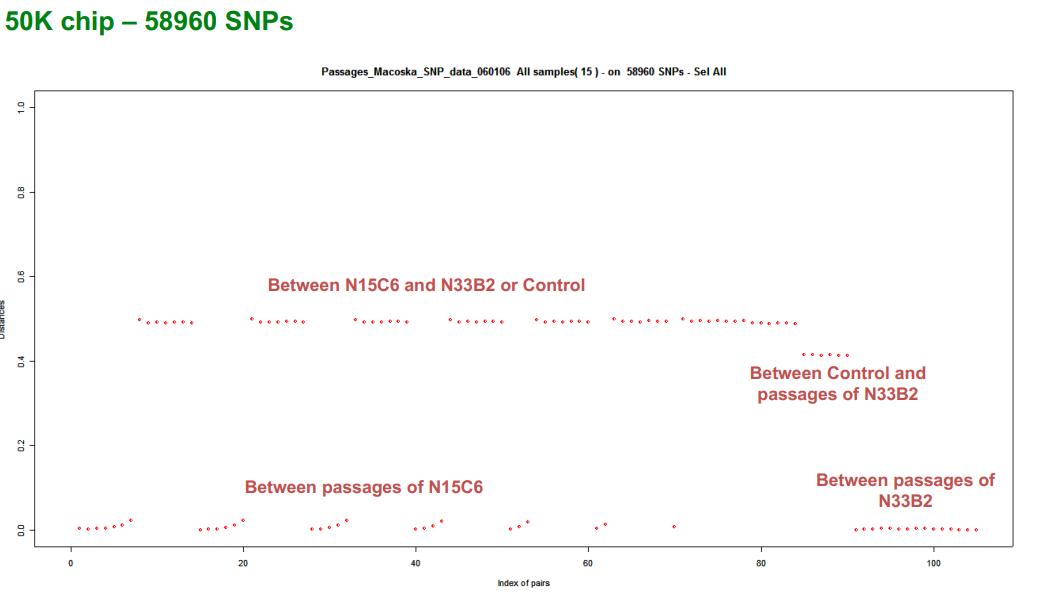
\includegraphics[width=0.4\textwidth]{50k.png}\quad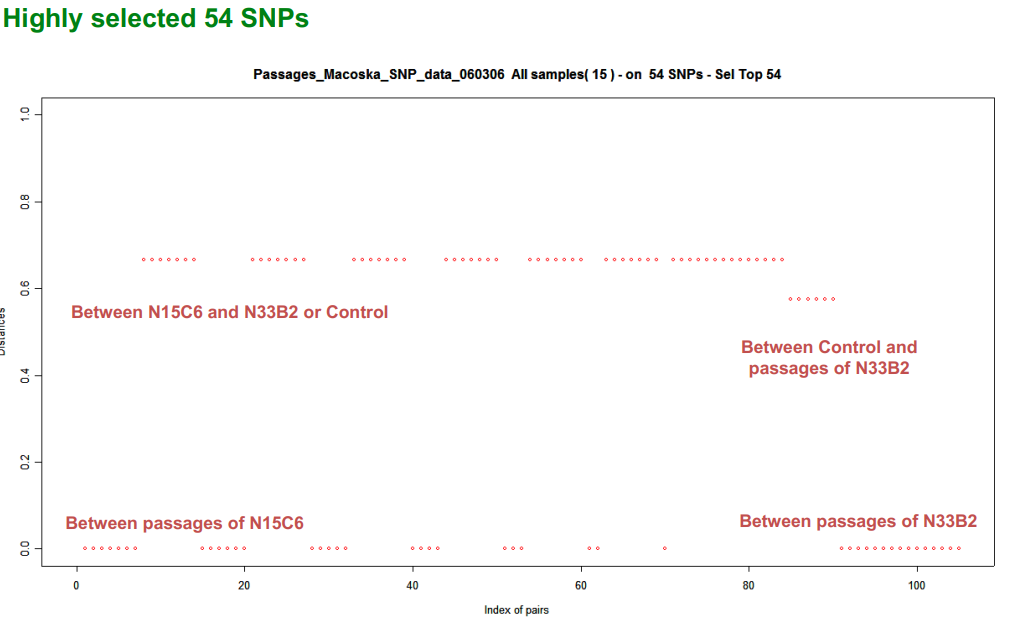
\includegraphics[width=0.4\textwidth]{54_snps.PNG}
			\caption{Genetic distance between cell line passages}
			\label{fig:cell_lines}
		\end{figure}

		In the example \ref{fig:cell_lines}, two types of prostate cell lines which underwent multiple passages were used:

		\begin{multicols}{2}
			\begin{itemize}
				\item $N15C6$ from passages from $48$ to $63$.
				\item $N33B2$ from passages from $21$ to $39$.
			\end{itemize}
		\end{multicols}

		The cell lines were profiled with a SNPs array and a genetic fingerprinting test was performed.
		All passages of each cell lines were compared with all other passages.
		All passages from the same cell line should be classified as similar in the test.
		However the results obtained using the full array of SNPs (50k), showed that some pairs which should be exactly identical are different.
		They can be seen on the bottom-left of \ref{fig:cell_lines}.
		Using only $54$ SNPs this distance is not detectable.
		This increased distance is due to a major difference for certain passages with respect to the initial one on chromosome $11$ of $N15C6$.
		This is due to the insertion in chromosome $11$ of a viral sequence to immortalize the cell line.

		\subsubsection{Investigating individual relatedness}
		The HapMap consortium sequenced hundreds of individuals and trios for different ethnicities and also used trios.
		Trio sequencing is a technique which involves the sequencing of the genome of mother, father and their child.
		Trios provide major information of haplotype blocks and for identifying regions related to inheritance.

		\begin{figure}[H]
			\centering
			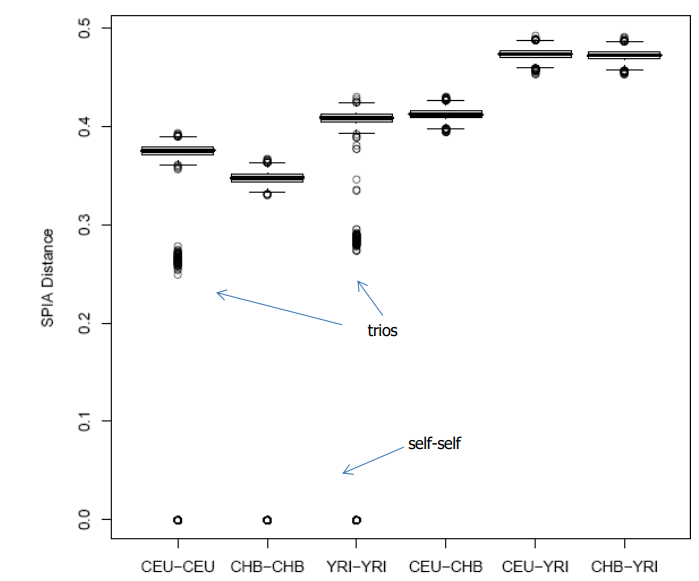
\includegraphics[width = 0.7\textwidth]{relatedness.PNG}
			\caption{Trio genotype distance}
			\label{fig:trios}
		\end{figure}

		Figure \ref{fig:trios} depicts the genetic distance of individuals computed by the SPIA Assay.
		Self-self pairs have a genetic distance of $0$.
		Each ethnicity has an average genetic distance different from the global one and trios have a lower distance from individual from the same ethnicity.
		Different in MAF in population could explain differences in distance among mixed samples.
		This shows how this type of test can be used for paternity tests of for forensic science.

	\subsection{Genetic structure of the human population}
	One relevant aspect of the human genome is that it contains everything needed to learn about the genetic structure of the human population.
	Understanding the genetic structure of human populations is of fundamental interest to medial, forensic and anthropological sciences.
	Knowing the genetic substructure of data is important because:

	\begin{multicols}{2}
		\begin{itemize}
			\item The goal of association studies is to identify DNA variants that affect disease risk or other traits of interest.
				However, association studies can be confounded by differences in ancestry.
			\item Misleading results could arise if individuals selected as disease cases have different ancestry, on average, than healthy controls.
				If in a study all controls are of the same ethnicity and the test is done on an individual of a different ethnicity than the test is biased.
			\item If GWAS study using a specific ethnicity a worldwide marker for susceptibility for a molecule or disease cannot be trusted.
		\end{itemize}
	\end{multicols}

In medicine and in the study of human evolution is important to track the genetic background of individuals that are involved in studies in order to understand if the individuals are form a homogeneous population or from genetically distant ones.
More and more, clinical studies must have declarations of the checks and interpretation of the data of the genetic background of the individuals present in the study.
It is very important to come to results for which we know exactly what is the applicability.
To avoid spurious results, association studies often restrict their focus to a single continental group.
Advances in high-throughput genotyping technology have improved the understanding of global patterns of human genetic variation and suggest the potential to use large sample sets to uncover variation among closely spaced populations.
One important piece of information to consider when developing methods to understand the genetic structure of a population is to think in term of variance, which is also relevant for human diseases.
Many SNPs have different MAFs in different populations and those could be used to infer the individual genetic background in terms of origins.
The easiest mathematical approach to assess how well SNPs can distinguish ethnicity is by using \textbf{Principal Component Analysis (PCA)}.
By running a very simple PCA on a set of SNPs including SNPs with different MAF in different populations different ethnical groups can be distinguished.

		\subsubsection{Genes mirror geography in Europe}
		$500k$ single nucleotide polymorphism array was used to genotype samples.
		Information about the country of origin of grandparents, parents and other relatives was used to determine the geographical location that best represents each individual ancestry.
		They run a combined study where they used a supervised search to find the best SNPs to make inference and then they tested it on another set of individuals.
		By using high confidence data (individuals with high confidence origin data) and by using the genotypes of highly informative SNPs for specific region-related inheritance, they were able to rebuild the map of some of the countries in Europe \ref{fig:PCA_countries}.

		\begin{figure}[H]
			\centering
			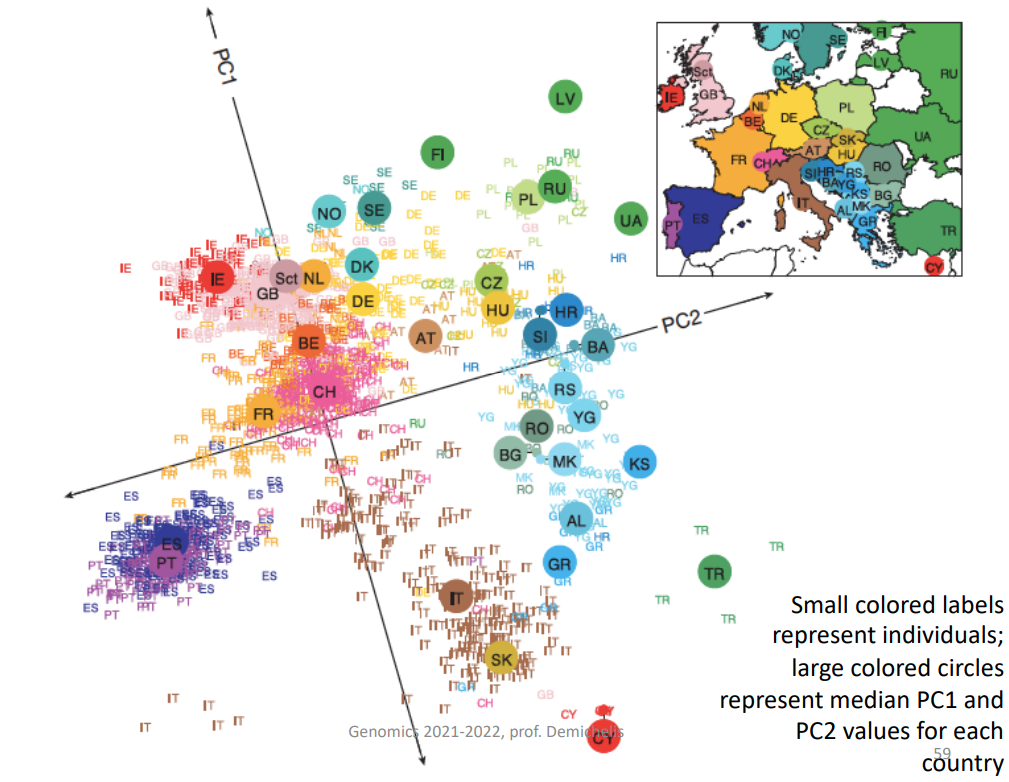
\includegraphics[width=0.7\textwidth]{population.PNG}
			\caption{\label{fig:PCA_countries}}
		\end{figure}

		Properly selecting variants it should be possible to distinguish individuals coming from different countries.
		SNPs were selected following the genetic fingerprinting approach, adding for SNPs with different MAF in different population.
		More dense and distant clusters could be due to the fact that SNPs selected are typical for that area and are able to maximize the difference with respect to it.

		\begin{figure}[H]
			\centering
			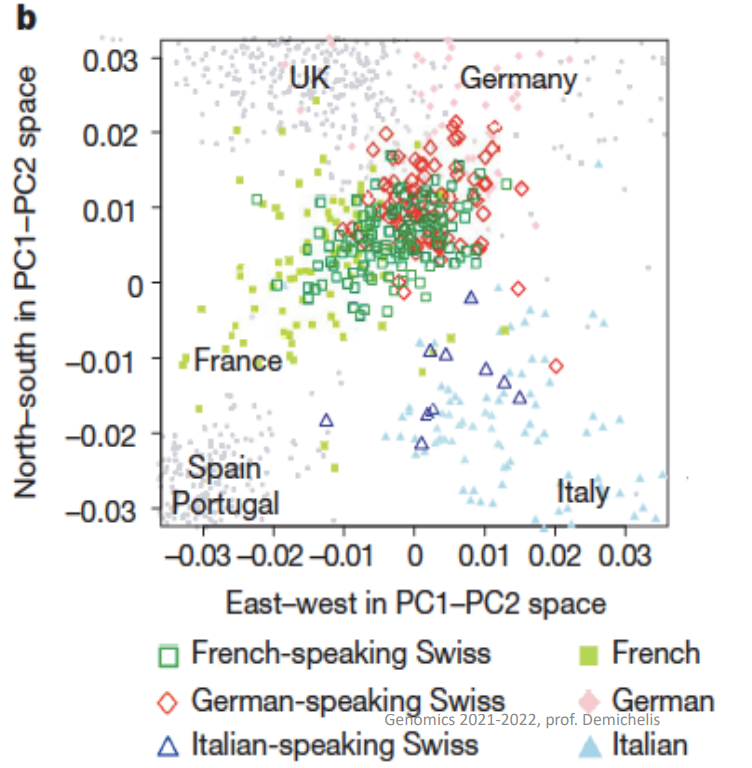
\includegraphics[width=0.5\textwidth]{swiss.PNG}
			\caption{\label{fig: PCA_swiss}}
		\end{figure}

		Focusing on Switzerland, they could even make inference on the linguistic canton \ref{fig: PCA_swiss}.
		It is possibly true that in country where some regions have very different habits might lead to have similar genetic fingerprint.
		Moreover low-frequency alleles tend to be the result of a recent mutation and are expected to geographically cluster around the location at which the mutation first arose.
		Hence, they can be highly informative about the fine-scale population structure.
		Despite low average levels of genetic differentiation among Europeans, close correspondence between genetic and geographic distances was found.
		When mapping the genetic basis of a disease phenotype, spurious associations can arise if genetic structure is not properly accounted for.
